\chapter{Regler}
Das Kapitel arbeitet sich von der untersten Reglerebene am Rad bis zum übergeordneten Lageregler vor und folgt damit der Signalkette aus Abbildung Konzept in umgekehrter Richtung. Den Anfang macht der Drehzahlregler, der an jedem der drei Räder dafür sorgt, dass die vorgegebene Solldrehzahl anliegt. Da Gewerk 2 jedoch keine Raddrehzahlen, sondern eine Sollgeschwindigkeit des Roboters liefert, ist eine Transformation von Roboter in Motorkoordinaten nötig. Damit sind alle Bausteine für die Vektorfahrweise beisammen. Für die Positionsfahrweise kommt eine weitere Ebene hinzu: Die gemessene Position liegt in Weltkoordinaten vor und muss in das Roboterkoordinatensystem überführt werden. Darauf setzt schließlich der Lageregler auf, dessen Parameter über ein Gain-Scheduling an die jeweilige Situation angepasst werden, um eine zuverlässige Fahrt sicherzustellen.
\section{Drehzahlregler}
Der Drehzahlregler sorgt dafür, dass eine vorgegebene Sollgeschwindigkeit des Roboters auf die Motorbewegung der einzelnen Motoren übersetzt wird und korrekt umgesetzt wird. Der Drehzahlreger wird in TwinCAT als Funktionsbaustein umgesetzt. Als Eingangsgrößen werden Sollgeschwindigkeiten in X,Y, und $\theta$ im Roboterkoordinatensystembenötigt. Außerdem werden die Istgeschwindigkeiten der einzelnen Motoren an den Eingang zurückgeführt. Der Ausgang ist das Geschwidigkeitessignal für die einzelnen drei Motoren. Abbildung \ref{fig:Drehzahlregler_BB} zeigt den Drehzahlregler als Blackbox mit Eingangs- und Ausgangssignalen.

\begin{figure}[H]
    \centering
    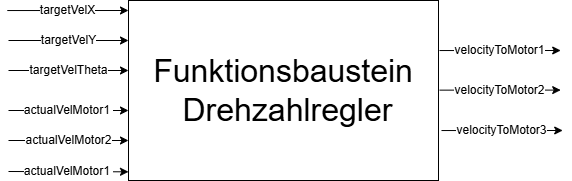
\includegraphics[width=0.8\textwidth]{_Bilder/Drehzahlregler_BB.png}
    \caption{Drehzahlregler als Blackbox mit Eingangs- und Ausgangssignalen}
    \label{fig:Drehzahlregler_BB}
\end{figure}

\textbf{TargetVelocity}\\
Die Target Velocity ist die Sollgeschwidigkeit des Roboters im Koordinatensystem des Roboters. Sie wird in $\frac{m}{s}$ angegeben und besteht aus drei voneinander unabhängigen Komponenten: X, Y und $\theta$. Die X-Komponente beschreibt die Geschwindigkeit in Vorwärtsrichtung, die Y-Komponente die Geschwindigkeit in Querrichtung und die $\theta$-Komponente die Winkelgeschwindigkeit um die Z-Achse. Durch Überlagerung der Bewegungen ist der Roboter in der Lage sich in alle Richtungen im Raum zu bewegen.
\textbf{VelWheel}\\
VelWheel1, -2 und -3 ist die Istgeschwindigkeit der einzelnen Motoren. Sie wird auch in $\frac{m}{s}$ angegeben. Die Berechnung erfolgt über den Encoder des Motors und den Radumfang mit folgender Formel:
\begin{equation}
    \text{VelWheel1} = -\frac{n_{1,\text{fromMotor}}}{n_{\text{max,KlemmeDrehzahlMessung}}} \cdot \frac{n_{\text{max,MotorRPM}}}{60} \cdot \ddot{u} \cdot 2\pi \cdot r_{\text{Wheel}}
\end{equation}

\noindent Dabei bezeichnen:
\begin{itemize}
    \item $n_{1,\text{fromMotor}}$ -- Rohwert der Drehzahlmessung an der Motorklemme (vorzeichenbehaftet).
    \item $n_{\text{max,KlemmeDrehzahlMessung}} = 10\,000$ -- Wert, den die Klemme bei maximaler Motordrehzahl zurückliefert (Skalierungsreferenz der Messung).
    \item $n_{\text{max,MotorRPM}} = 3600\ \text{rpm}$ -- maximale Motordrehzahl. Zusammen mit dem vorherigen Term wird der Rohwert auf eine tatsächliche Drehzahl in Umdrehungen pro Minute umgerechnet; die Division durch $60$ wandelt diese in Umdrehungen pro Sekunde um.
    \item $\ddot{u} = 0{,}0625$ -- Getriebeübersetzung zwischen Motor- und Raddrehzahl (Ausgangsdrehzahl = Motordrehzahl $\cdot\ \ddot{u}$).
    \item $r_{\text{Wheel}} = 40\ \text{mm}$ -- Radradius. Über $2\pi \cdot r_{\text{Wheel}}$ wird die Raddrehzahl (in Umdrehungen/s) in eine Umfangsgeschwindigkeit umgerechnet.
\end{itemize}

\noindent Die Einheit von $r_{\text{Wheel}}$ ist Millimeter, somit ist die Einheit von $\text{VelWheel} \text{mm/s}$.\\
\textbf{VelocityToMotor}\\
VelocityToMotor1, -2 und -3 ist das jeweilige Ausgangssignal des Drehzahlreglers an die drei Motoren. Da die Motoren als Sollwert keinen Geschwindigkeitswert in $\text{mm/s}$, sondern einen skalierten Integerwert erwarten, muss $\text{VelWheel}$ vor der Ausgabe mit einem Skalierungsfaktor multipliziert werden. Die Berechnung erfolgt mit folgender Formel:

\begin{equation}
    \text{VelocityToMotor1} = \text{VelWheel1} \cdot \text{skalPos}
\end{equation}

\noindent Dabei bezeichnen:
\begin{itemize}
    \item $\text{VelWheel1}$ -- Istgeschwindigkeit des Motors in $\text{mm/s}$ (siehe oben).
    \item $\text{skalPos} = 34{,}7668668\ \left[\dfrac{1}{\text{mm/s}}\right]$ -- Skalierungsfaktor, der die Geschwindigkeit in $\text{mm/s}$ auf den vom Motor erwarteten Integer-Wertebereich abbildet. Er berechnet sich aus dem Verhältnis von maximalem Ausgabewert zu maximal erreichbarer Geschwindigkeit:
    \begin{equation}
        \text{skalPos} = \frac{\text{MaxValue}}{\text{MaxVelocity}}
    \end{equation}
    \item $\text{MaxValue} = 32767$ -- maximaler darstellbarer Ausgabewert (Wertebereich eines vorzeichenbehafteten 16-Bit-Integers).
    \item $\text{MaxVelocity} = 942\ \text{mm/s}$ -- maximal erreichbare Geschwindigkeit des Rades, berechnet aus dem Raddurchmesser $D$, der maximalen Motordrehzahl $n$ und der Getriebeübersetzung:
    \begin{equation}
        \text{MaxVelocity} = \frac{D \cdot \pi \cdot n}{16 \cdot 60}
    \end{equation}
    \item $D$ -- Raddurchmesser in mm.
    \item $n$ -- maximale Motordrehzahl in rpm.
    \item $16$ -- Getriebeübersetzung (Motor- zu Raddrehzahl, entspricht $\ddot{u} = \tfrac{1}{16} = 0{,}0625$).
    \item $60$ -- Umrechnungsfaktor von Minuten auf Sekunden.
\end{itemize}

\noindent Da $\text{VelWheel1}$ in $\text{mm/s}$ und $\text{skalPos}$ in $\tfrac{1}{\text{mm/s}}$ angegeben sind, ist $\text{VelocityToMotor1}$ dimensionslos und stellt den direkten Sollwert für den Motorregler dar.
\section{Koordinatentransformation Roboter -> Motoren}
\section{Koordinatentransformation Welt -> Roboter}
\section{Positionsregler}
\section{Auswertung}
\subsection{Vektorfahrweise}
\subsection{Positionsfahrweise}


